\chapter{Wyniki eksperymentu}
\label{c5}

Dany rozdział zawiera wyniki z przeprowadzonych badań oraz wnioski. Każda aplikacja, która została napisana została przestawiona i opisana z różnych perespektyw. Na końcu rozdziału zostały przedstawione wady i zalety obu podejść.

\section{Stworzone aplikacje}

Aplikacje zostały najpierw stworzone w App Inventorze, a następnie zostały przepisane na język Java.

\subsection{Sortowanie}

Aplikacja polega na wygenerowaniu listy losowych elementów, a następnie posortowaniu jej. Do sortowania został użyty prosty algorytm sortowania przez wybieranie \english{Selection Sort}.

\begin{figure}[th] 
\centering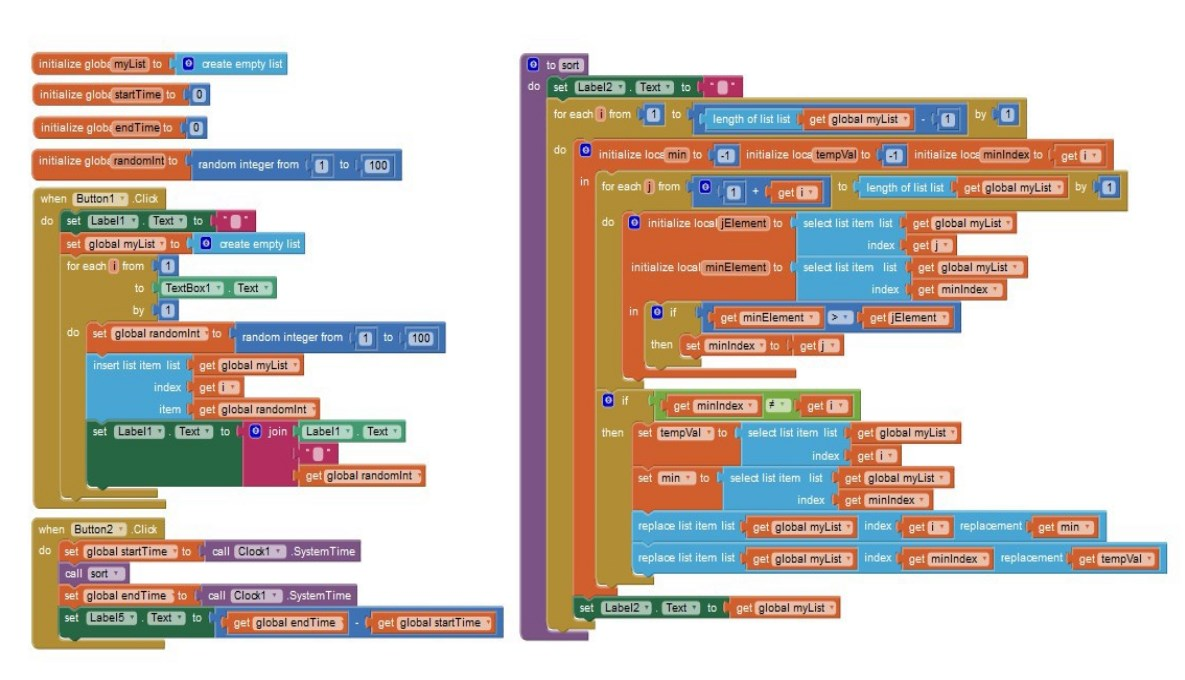
\includegraphics[width=10cm]{figures/apps/sort}
\caption{Aplikacja sortująca - App Inventor}
\end{figure}

Na powyższym rysunku widać bloki potrzebne do stowrzenia aplikacji w App Inventorze. Bez głębszej analizy zrozumienie działania bloków, może okazać się kłopotliwe. Jest to prosty algorytm, a napisanie go za pomocą dostępnych bloków okazało się skomplikowane. Można sobie łatwo wyobrazić, że napisanie bardziej skomplikowanego algorytmu byłoby bardzo nieczytelne. Ilość użytych bloków zdecydowanieby wzrosła, dodatkowo utrzymanie takiej aplikacji niesie za sobą wysokie koszty wprowadzenia nowych osób do jej rozwijania.

Sortowanie napisanie w javie jest zrozumiałe dla każdego programisty. Do sortowania została użyta lista, jako odpowiednik listy w App Inventorze, nie ma tam dostępnych tablic.


\begin{lstlisting}
 void sort(List<Integer> list){
        for(int i =0;i<list.size()-1;i++){
            int index = i;
            for(int j=i+1;j<list.size();j++){
                if(list.get(j) < list.get(index) ){
                    index = j;
                }
            }
            if(index != i){
                int tmp = list.get(i);
                list.set(i,list.get(index));
                list.set(index,tmp);
            }
        }
    }
\end{lstlisting}

W algorytmach bardzo ważna jest wydajność. Oba algorytmy działają w ten sam sposób, jednak wydajność sortowania listy napisanej w Javie jest zdecydowanie wyższa. Można to zaobserwować na poniższym wykresie. Przesortowanie bardzo małej liczby elementów zajmuje App Inventorowi bardzo dużo czasu. Przy 25 elementach czas sortowania przekroczył 1 sekundę. Jest to bardzo słaby wynik w porównaniu do sortowania napisanego w Javie. Średnio czas sortowania był 2 tysiące razy mniejszy! Na danym wykresie została zastosowana skala logarytmiczna, aby zobaczyć różnicę.

\begin{figure}[htbp]
\centering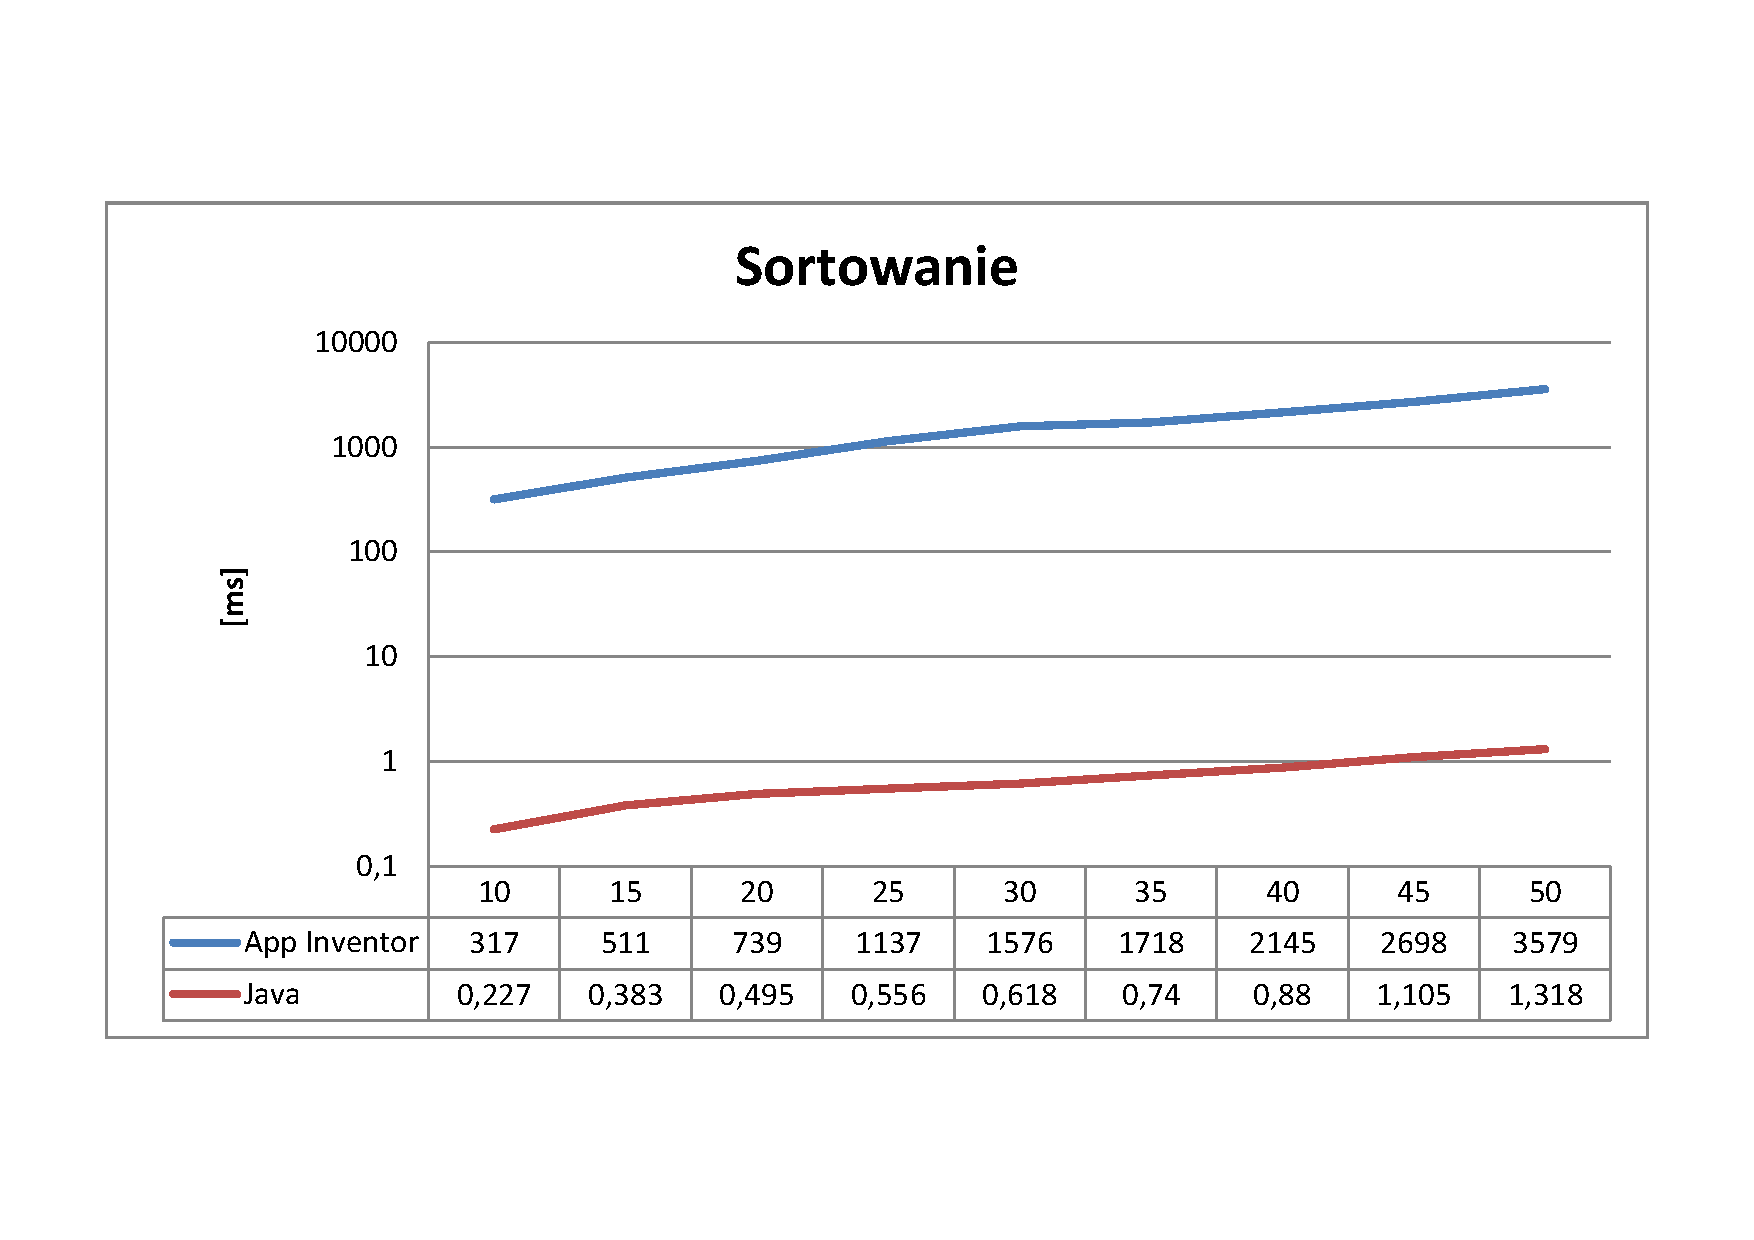
\includegraphics[width=10cm]{figures/apps/sortChart}
\caption{Wykres przedstawiający czas sortowania}
\end{figure}

Napisanie tej aplikacji w Javie nie było żadnym problemem. Bardzo łatwo było zdebugować kod i sprawdzić jego poprawność. Stworzenie tej samej aplikacji w App Inventorze nie było trywialne.


\subsection{Akcelerometr}

Kolejną aplikacją jest wykorzystująca akcelerometr. Odczytuje ona dane z akcelerometru, a następnie wyświetla je na ekran telefonu, z zadaną częstotliwością. O ile 





\section{Zalety programowania wizualnego}

\section{Wady programowania wizualnego}
